\pdfinfoomitdate=1
\pdftrailerid{}
\pdfsuppressptexinfo=-1
\documentclass[10pt,a4paper]{article}
\usepackage{cmap}
\usepackage[margin=1.8cm,headheight=14pt,headsep=10pt]{geometry}
\usepackage[leqno]{amsmath}
\usepackage{amssymb,booktabs,longtable,array,ragged2e,multicol,multirow,xcolor,fancyhdr,tikz}
\definecolor{linkblue}{rgb}{0.08,0.33,0.58}
\usepackage[colorlinks=true,linkcolor=linkblue,urlcolor=linkblue,citecolor=linkblue,
  filecolor=linkblue,linktoc=all,pdfborder={0 0 0},bookmarksnumbered=true]{hyperref}
\setlength{\parindent}{0pt}\setlength{\parskip}{4pt}
\setcounter{secnumdepth}{2}\setcounter{tocdepth}{2}
\definecolor{partshade}{gray}{0.9}
\usepackage{nicefrac}
\definecolor{parttitle}{HTML}{295A2C}
\definecolor{parttitlelight}{HTML}{6C9F6D}
\makeatletter
\renewcommand\section{\@startsection{section}{1}{\z@}{-3ex plus -1ex minus -.2ex}%
  {1.2ex plus .2ex}{\normalfont\large\sffamily\bfseries\color{parttitle}}}
\renewcommand\subsection{\@startsection{subsection}{2}{\z@}{-2.5ex plus -1ex minus -.2ex}%
  {.8ex plus .2ex}{\normalfont\sffamily\bfseries\color{parttitle}}}
\renewcommand\subsubsection{\@startsection{subsubsection}{3}{\z@}{-2ex plus -1ex minus -.2ex}%
  {.6ex plus .2ex}{\normalfont\small\sffamily\bfseries\color{parttitle}}}
\renewcommand\paragraph{\@startsection{paragraph}{4}{\z@}{1.5ex plus .5ex minus .2ex}{-1em}%
  {\normalfont\small\sffamily\bfseries\color{parttitle}}}
\renewcommand\tagform@[1]{\maketag@@@{\textsf{\bfseries\footnotesize (#1)}}}
\renewcommand*\l@part[2]{\par\addvspace{1.6ex}\noindent{\sffamily\bfseries #1}\hfill
  {\sffamily\bfseries #2}\par\nobreak}
\newcommand\tocnumber{1.8em}
\newcommand\tocline[4]{\par{\rightskip \tocnumber plus 1fil\relax\parfillskip -\rightskip
  \noindent\hangindent\dimexpr#1+#2\relax\hspace*{#1}%
  \@tempdima #2{\sffamily\small #3}\nobreak\leaders\hbox{$\m@th\mkern 4.5mu\hbox{.}%
  \mkern 4.5mu$}\hfill\nobreak\hbox to \tocnumber{\hfil\sffamily\small #4}\par}}
\renewcommand*\l@section[2]{\tocline{0em}{2.2em}{#1}{#2}}
\renewcommand*\l@subsection[2]{\tocline{2.2em}{2.6em}{#1}{#2}}
\newcommand\contentspage{{\setlength{\columnsep}{24pt}\begin{multicols}{2}\@starttoc{toc}%
  \end{multicols}}}
\newcounter{docpart}\@addtoreset{section}{docpart}
\renewcommand\thesection{\ifnum\value{docpart}>0 \arabic{docpart}.\fi\arabic{section}}
\renewcommand\theHsection{\arabic{docpart}.\arabic{section}}
\newcommand\partnumber[1]{#1\enspace}
\pdfstringdefDisableCommands{\def\partnumber#1{#1 }}
\newcommand{\partbox}[1]{\par\addvspace{12pt}\refstepcounter{docpart}\phantomsection
  \addcontentsline{toc}{part}{\protect\partnumber{\thedocpart}#1}%
  \noindent\colorbox{partshade}{\makebox[%
  \dimexpr\textwidth-2\fboxsep\relax]{\rule[-6pt]{0pt}{20pt}\Large\sffamily\bfseries%
  \textcolor{parttitle}{\thedocpart\quad #1}}}\par\nobreak\@nobreaktrue\addvspace{2pt}}
\newmarks\LTstartmarks\newcount\LTstartcount
\let\LT@startplain\LT@start
\def\LT@start{\global\advance\LTstartcount\@ne\LT@startplain
  \marks\LTstartmarks{\the\LTstartcount}}
\newmarks\LTgroupmarks
\newcount\LTspacebreak\LTspacebreak=-1
\newcount\LTrulebreak\LTrulebreak=-2
\def\grouprule#1#2{\noalign{\marks\LTgroupmarks{\the\belowrulesep}\nobreak\vskip#1%
  \vskip\aboverulesep}\multispan\LT@cols\unskip{\leaders\hrule\@height#2\hfill\kern\z@}\cr
  \noalign{\penalty\LTrulebreak\vskip\belowrulesep\global\@lastruleclass\z@}}
\def\groupspace#1{\noalign{\marks\LTgroupmarks{\the\dimexpr#1\relax}\penalty\LTspacebreak
  \vskip#1\global\@lastruleclass\z@}}
\def\LT@unskips{\unskip\unpenalty\unskip\unpenalty\unskip\unpenalty\unskip\unpenalty}
\def\LT@groupcut{\ifnum\outputpenalty=\LTrulebreak
  \setbox\@cclv\vbox{\unvbox\@cclv\setbox\z@\lastbox\LT@unskips}\fi}
\def\LT@groupjoin{\ifnum\outputpenalty=\LTspacebreak\vskip-\botmarks\LTgroupmarks\relax\fi
  \ifnum\outputpenalty=\LTrulebreak\vskip-\botmarks\LTgroupmarks\relax\fi}
\let\LT@outputplain\LT@output
\def\LT@output{\ifnum\outputpenalty<-\@Mi\LT@outputplain\else
  \edef\LT@marka{\botmarks\LTstartmarks}\edef\LT@markb{\the\LTstartcount}%
  \ifx\LT@marka\LT@markb\LT@groupcut\LT@outputplain\LT@groupjoin
  \else\setbox\LT@head\box\voidb@x\LT@outputplain\fi\fi}
\makeatother
\newcommand{\needspace}[1]{\par\penalty-100\begingroup\dimen0=#1\relax\dimen2=\pagegoal
  \advance\dimen2-\pagetotal\ifdim\dimen0>\dimen2\relax\ifdim\dimen2>0pt\vfil\break\fi\fi
  \endgroup}
\numberwithin{equation}{section}
\pagestyle{fancy}\fancyhf{}
\renewcommand{\headrulewidth}{0pt}
\renewcommand{\sectionmark}[1]{\markright{\thesection\enspace #1}}
\renewcommand{\subsectionmark}[1]{}
\fancyhead[R]{\small\textsc{\rightmark}\quad\thepage}
\fancypagestyle{plain}{\fancyhf{}\fancyfoot[C]{\small\thepage}}
\definecolor{atlasI}{HTML}{991A1A}\definecolor{atlasIl}{HTML}{EC6B60}
\definecolor{atlasII}{HTML}{295A2C}\definecolor{atlasIIl}{HTML}{6C9F6D}
\definecolor{atlasIII}{HTML}{7A1466}\definecolor{atlasIIIl}{HTML}{D66EBC}
\definecolor{atlasIV}{HTML}{9B690B}\definecolor{atlasIVl}{HTML}{F2A618}
\makeatletter
\newcommand\atlas@full{%
\fill[atlasIII] (0.0394,0.0163) -- (0.3978,0.0163) arc[start angle=0.668, end angle=13.836, radius=1.3979] -- cycle;
\fill[atlasI] (-0.0163,0.0394) -- (-0.0163,0.3978) arc[start angle=90.668, end angle=103.836, radius=1.3979] -- cycle;
\fill[atlasIV] (-0.0394,-0.0163) -- (-0.3978,-0.0163) arc[start angle=-179.332, end angle=-166.164, radius=1.3979] -- cycle;
\fill[atlasII] (0.0163,-0.0394) -- (0.0163,-0.3978) arc[start angle=-89.332, end angle=-76.164, radius=1.3979] -- cycle;
\fill[atlasIIIl] (0.0163,0.0394) -- (0.3343,0.3573) arc[start angle=76.164, end angle=89.332, radius=1.3979] -- cycle;
\fill[atlasIl] (-0.0394,0.0163) -- (-0.3573,0.3343) arc[start angle=166.164, end angle=179.332, radius=1.3979] -- cycle;
\fill[atlasIVl] (-0.0163,-0.0394) -- (-0.3343,-0.3573) arc[start angle=-103.836, end angle=-90.668, radius=1.3979] -- cycle;
\fill[atlasIIl] (0.0394,-0.0163) -- (0.3573,-0.3343) arc[start angle=-13.836, end angle=-0.668, radius=1.3979] -- cycle;
\fill[atlasIIIl] (0.4304,0.0163) -- (0.9598,0.0163) arc[start angle=46.637, end angle=73.849, radius=1.3979] arc[start angle=13.862, end angle=0.653, radius=1.4305] -- cycle;
\fill[atlasIl] (-0.0163,0.4304) -- (-0.0163,0.9598) arc[start angle=136.637, end angle=163.849, radius=1.3979] arc[start angle=103.862, end angle=90.653, radius=1.4305] -- cycle;
\fill[atlasIVl] (-0.4304,-0.0163) -- (-0.9598,-0.0163) arc[start angle=-133.363, end angle=-106.151, radius=1.3979] arc[start angle=-166.138, end angle=-179.347, radius=1.4305] -- cycle;
\fill[atlasIIl] (0.0163,-0.4304) -- (0.0163,-0.9598) arc[start angle=-43.363, end angle=-16.151, radius=1.3979] arc[start angle=-76.138, end angle=-89.347, radius=1.4305] -- cycle;
\fill[atlasIII] (0.0163,0.4304) arc[start angle=89.347, end angle=76.138, radius=1.4305] arc[start angle=16.151, end angle=43.363, radius=1.3979] -- cycle;
\fill[atlasI] (-0.4304,0.0163) arc[start angle=179.347, end angle=166.138, radius=1.4305] arc[start angle=106.151, end angle=133.363, radius=1.3979] -- cycle;
\fill[atlasIV] (-0.0163,-0.4304) arc[start angle=-90.653, end angle=-103.862, radius=1.4305] arc[start angle=-163.849, end angle=-136.637, radius=1.3979] -- cycle;
\fill[atlasII] (0.4304,-0.0163) arc[start angle=-0.653, end angle=-13.862, radius=1.4305] arc[start angle=-73.849, end angle=-46.637, radius=1.3979] -- cycle;
\fill[atlasIII] (0.9997,0.0232) arc[start angle=1.329, end angle=44.066, radius=1] -- (0.3973,0.3742) arc[start angle=73.875, end angle=45.664, radius=1.4305] -- cycle;
\fill[atlasI] (-0.0232,0.9997) arc[start angle=91.329, end angle=134.066, radius=1] -- (-0.3742,0.3973) arc[start angle=163.875, end angle=135.664, radius=1.4305] -- cycle;
\fill[atlasIV] (-0.9997,-0.0232) arc[start angle=-178.671, end angle=-135.934, radius=1] -- (-0.3973,-0.3742) arc[start angle=-106.125, end angle=-134.336, radius=1.4305] -- cycle;
\fill[atlasII] (0.0232,-0.9997) arc[start angle=-88.671, end angle=-45.934, radius=1] -- (0.3742,-0.3973) arc[start angle=-16.125, end angle=-44.336, radius=1.4305] -- cycle;
\fill[atlasIIIl] (0.0232,0.9997) arc[start angle=44.336, end angle=16.125, radius=1.4305] -- (0.6955,0.7185) arc[start angle=45.934, end angle=88.671, radius=1] -- cycle;
\fill[atlasIl] (-0.9997,0.0232) arc[start angle=134.336, end angle=106.125, radius=1.4305] -- (-0.7185,0.6955) arc[start angle=135.934, end angle=178.671, radius=1] -- cycle;
\fill[atlasIVl] (-0.0232,-0.9997) arc[start angle=-135.664, end angle=-163.875, radius=1.4305] -- (-0.6955,-0.7185) arc[start angle=-134.066, end angle=-91.329, radius=1] -- cycle;
\fill[atlasIIl] (0.9997,-0.0232) arc[start angle=-45.664, end angle=-73.875, radius=1.4305] -- (0.7185,-0.6955) arc[start angle=-44.066, end angle=-1.329, radius=1] -- cycle;
}
\newcommand\atlas@draw[2]{\begin{tikzpicture}[x=\dimexpr(#1)/2\relax,y=\dimexpr(#1)/2\relax]
\useasboundingbox (-1,-1) rectangle (1,1);#2\end{tikzpicture}}
\newcommand\atlas@volume[1]{{%
\colorlet{atlasI}{parttitle}\colorlet{atlasIl}{parttitlelight}%
\colorlet{atlasII}{parttitle}\colorlet{atlasIIl}{parttitlelight}%
\colorlet{atlasIII}{parttitle}\colorlet{atlasIIIl}{parttitlelight}%
\colorlet{atlasIV}{parttitle}\colorlet{atlasIVl}{parttitlelight}%
#1}}
\newcommand\atlasmark[1]{\atlas@draw{#1}{\atlas@full}}
\newcommand\volumemark[1]{\atlas@volume{\atlasmark{#1}}}
\makeatother
\fancypagestyle{opening}{\fancyhf{}\fancyfoot[C]{\small\thepage}%
  \fancyhead[L]{\smash{\raisebox{-9.5mm}{\volumemark{12mm}}}}}
\hypersetup{pdftitle={S6b: Point Group Atlas, volume II: double point groups}, pdfauthor={Victor V. Albert}, pdfsubject={Point Group Atlas double record S6b, schema point-group-atlas/double/section/1}}
\fancyhead[L]{\small $\grp{S_{6}}\secondclass$}
\DeclareMathAlphabet{\mathelt}{OT1}{cmss}{m}{sl}
\DeclareSymbolFont{eltgreek}{OML}{cmssm}{m}{it}
\DeclareMathSymbol{\eltsigma}{\mathord}{eltgreek}{"1B}
\DeclareSymbolFont{eltletters}{OT1}{cmss}{m}{sl}
\DeclareMathSymbol{g}{\mathalpha}{eltletters}{`g}
\DeclareMathSymbol{h}{\mathalpha}{eltletters}{`h}
\DeclareMathSymbol{Q}{\mathalpha}{eltletters}{`Q}
\DeclareMathSymbol{R}{\mathalpha}{eltletters}{`R}
\DeclareMathSymbol{\xi}{\mathord}{eltgreek}{"18}
\newcommand{\eltfont}[1]{{\let\sigma\eltsigma\mathelt{#1}}}
\newcommand{\grp}[1]{\mathsf{#1}}
\newcommand{\irr}[1]{\text{\normalfont\scshape #1}}
\newcommand{\conjpair}[1]{{}^{#1}}
\newcommand{\detbox}[1]{{\setlength{\fboxsep}{1pt}\fbox{#1}}}
\newcommand{\cls}[1]{\eltfont{#1}}
\newcommand{\comp}[1]{\eltfont{#1}}
\newcommand{\elt}[1]{\eltfont{#1}}
\newcommand{\hmname}[1]{#1}
\newcommand{\conwayname}[1]{#1}
\newcommand{\ptag}[1]{\mathrm{#1}}
\newcommand{\orbital}[1]{\mathrm{#1}}
\newcommand{\dirprod}{\times}
\newcommand{\sdprod}{\rtimes}
\newcommand{\samecls}{\cong}
\newcommand{\nconj}[1]{{\scriptsize$\times#1$}}
\newcommand{\clsletter}[1]{\,{\scriptsize\color{black!55}#1}}
\newcommand{\Cyc}[1]{\grp{Z_{#1}}}
\newcommand{\Sym}[1]{\grp{Sym_{#1}}}
\newcommand{\dirvec}[3]{(#1, #2, #3)}
\newcommand{\grpindex}[2]{[#1 : #2]}
\newcommand{\iverson}[1]{[#1]}
\newcommand{\restr}[2]{#1\!\downarrow#2}
\newcommand{\Ind}[2]{\operatorname{Ind}_{#1}^{#2}}
\newcommand{\genidx}[2]{#1^{[\mathrm{#2}]}}
\newcommand{\pointr}{\mathbf{r}}
\newcommand{\unitaxis}{\hat{\mathbf{v}}}
\newcommand{\vv}{\mathbf{v}}
\newcommand{\iunit}{\mathrm{i}}
\newcommand{\expe}{\mathrm{e}}
\newcommand{\diff}{\mathrm{d}}
\newcommand{\goldenratio}{\varphi}
\newcommand{\rootunity}[1]{\zeta_{#1}}
\newcommand{\irrJ}[1]{D^{(#1)}}
\newcommand{\irrJp}[2]{D^{(#1,#2)}}
\newcommand{\repD}[1]{D^{#1}}
\newcommand{\wignerD}[1]{D^{#1}}
\newcommand{\wignerd}[1]{d^{#1}}
\newcommand{\irchar}[1]{\chi_{#1}}
\newcommand{\chiA}{\chi_{\grp{A}}}
\newcommand{\fsind}{\nu_{\mathrm{FS}}}
\newcommand{\conj}[1]{{#1}^{*}}
\newcommand{\diag}{\operatorname{diag}}
\newcommand{\trace}{\operatorname{tr}}
\newcommand{\irrprod}{\otimes}
\newcommand{\mult}{\kappa}
\newcommand{\intx}{\mu}
\newcommand{\cgnorm}{\mathcal{N}}
\newcommand{\jm}[2]{\bigl\lvert{}^{#1}_{\,#2}\bigr\rangle}
\newcommand{\cgket}[3]{\bigl\lvert{}^{#1}_{\,#2};#3\bigr\rangle}
\newcommand{\irket}[2]{\bigl\lvert{}^{#1}_{\,#2}\bigr\rangle}
\newcommand{\prodket}[2]{\lvert {#1}\,{#2}\rangle}
\newcommand{\ket}[1]{\lvert #1\rangle}
\newcommand{\cgc}[6]{\bigl\langle{}^{#1}_{\,#2}\,{}^{#3}_{\,#4}\bigm\vert{}^{#5}_{\,#6}\bigr\rangle}
\newcommand{\cgck}[7]{\bigl\langle{}^{#1}_{\,#2}\,{}^{#3}_{\,#4}\bigm\vert{}^{#5}_{\,#6};#7\bigr\rangle}
\newcommand{\cgcone}[3]{\langle #1\,#2\mid #3\rangle}
\newcommand{\irrangle}{\text{--}}
\newcommand{\vol}{\operatorname{vol}}
\newcommand{\fcell}{\mathcal{D}}
\newcommand{\fdomain}{\mathcal{F}}
\newcommand{\lensspace}[2]{\mathsf{L}(#1, #2)}
\newcommand{\twosphere}{\mathsf{S}^{2}}
\newcommand{\projplane}{\mathbb{R}\mathsf{P}^{2}}
\newcommand{\term}[2]{{}^{#1}#2}
\newcommand{\barred}[1]{\bar{#1}}
\newcommand{\Quat}[1]{\grp{Q_{#1}}}
\newcommand{\SL}[1]{\grp{SL}(2,#1)}
\newcommand{\secondclass}{\mathrm{b}}
\newcommand{\dmark}{{}^{d}}
\newcommand{\lift}[1]{\tilde{#1}}
\newcommand{\pauli}[1]{\sigma_{#1}}
\newcommand{\paulivec}{\vec{\sigma}}
\newcommand{\hairsp}{\mkern1mu}
\newenvironment{romanlist}{\begin{enumerate}%
\renewcommand{\labelenumi}{(\roman{enumi})}}%
  {\end{enumerate}}
\makeatletter
\newenvironment{irmatrix}[1]{\null\,\vcenter\bgroup\Let@\restore@math@cr\default@tag
  \baselineskip8\ex@ \lineskip3\ex@ \lineskiplimit\lineskip
  \ialign\bgroup\hfil$\m@th\scriptstyle##$\hfil&&\hskip#1\hfil$\m@th\scriptstyle##$\hfil\crcr}%
  {\crcr\egroup\egroup\,}
\makeatother
\newlength{\fillwidth}\newlength{\cellwidth}\newlength{\colwidth}
\newcommand{\cellmax}[1]{\settowidth{\cellwidth}{#1}%
  \ifdim\cellwidth>\colwidth\setlength{\colwidth}{\cellwidth}\fi}
\newcommand{\fillcap}{\ifdim\colwidth<\fillwidth\setlength{\fillwidth}{\colwidth}\fi}
\newcommand{\signbreak}{\penalty100\relax}
\begin{document}
\thispagestyle{opening}
\begin{center}
{\LARGE\sffamily\bfseries\color{parttitle}The $\grp{S_{6}}\secondclass$ subgroup of $\grp{Pin^{-}(3)}$}
\end{center}
\contentspage
\needspace{194pt}
\partbox{The group}
\section{Names and structure}\label{s:identification}
Conventions: \href{../../CONVENTIONS.pdf}{CONVENTIONS.pdf}, sections \href{../../../rotation/CONVENTIONS.pdf\#conv.0.1}{0.1}, \href{../../../rotation/CONVENTIONS.pdf\#conv.2}{2}, \href{../../CONVENTIONS.pdf\#conv.20}{20} and \href{../../CONVENTIONS.pdf\#conv.28}{28}.
{\small\begin{longtable}{@{}ll@{}}\toprule
\texttt{symbol} & \href{S6b.pdf}{$\grp{S_{6}}\secondclass$}\\
\texttt{image} & \href{../../../rotation/data/pdf/S6.pdf}{$\grp{S_{6}}$}\\
\texttt{section\symbol{95}of} & \href{2S6.pdf}{$\grp{2S_{6}}$}\\
\grouprule{0pt}{\lightrulewidth}
\texttt{order} & 6\\
\grouprule{0pt}{\lightrulewidth}
\texttt{normalizer} & \href{2Dinfh.pdf}{$\grp{2D_{\infty h}}$}\\
\texttt{centralizer} & \href{2Cinfh.pdf}{$\grp{2C_{\infty h}}$}, index 2 in the normalizer\\
\grouprule{0pt}{\lightrulewidth}
\texttt{altmann\symbol{95}T} & 14\\
\texttt{hermann\symbol{95}mauguin} & $\hmname{\bar{3}}\secondclass$\\
\bottomrule\end{longtable}}
\leavevmode\label{n:group.G}\label{n:element.inversion}\label{n:group.preimage}In this document, $\grp{G}$ is $\grp{S_{6}}\secondclass$, a section over $\grp{S_{6}}$ in $\grp{Pin^{-}(3)}$, which the covering map carries one to one onto $\grp{S_{6}}$ (\href{../../CONVENTIONS.pdf}{CONVENTIONS.pdf}, section \href{../../CONVENTIONS.pdf\#conv.27}{27}): its representations are those of $\grp{S_{6}}$, and its data at half-integer $J$ those of its preimage \href{2S6.pdf}{$\grp{2S_{6}}$} (\texttt{section\symbol{95}of}), with the spinor irreps renamed as the table below gives; in this table, \texttt{normalizer} and \texttt{centralizer} are taken in $\grp{Pin^{-}(3)}$.
A spinor irrep $\Delta$ of \href{2S6.pdf}{$\grp{2S_{6}}$} restricts to an irrep of $\grp{G}$, the irrep of $\grp{S_{6}}$ with the same characters on the elements of $\grp{G}$ (section~\ref{s:elements}):
\begin{center}\begin{tabular}{@{}lllllll@{}}\toprule
$\Delta$ & $\irr{a}_{3/2,\ptag{g}}$ & $\conjpair{1}\irr{e}_{1/2,\ptag{g}}$ & $\conjpair{2}\irr{e}_{1/2,\ptag{g}}$ & $\irr{a}_{3/2,\ptag{u}}$ & $\conjpair{1}\irr{e}_{1/2,\ptag{u}}$ & $\conjpair{2}\irr{e}_{1/2,\ptag{u}}$\\\midrule
on $\grp{G}$ & $\irr{a}_{\ptag{u}}$ & $\conjpair{2}\irr{e}_{\ptag{u}}$ & $\conjpair{1}\irr{e}_{\ptag{u}}$ & $\irr{a}_{\ptag{g}}$ & $\conjpair{2}\irr{e}_{\ptag{g}}$ & $\conjpair{1}\irr{e}_{\ptag{g}}$\\
\bottomrule\end{tabular}\end{center}
\needspace{103pt}
\section{Symmetry operations}\label{s:elements}
Conventions: \href{../../CONVENTIONS.pdf}{CONVENTIONS.pdf}, sections \href{../../../rotation/CONVENTIONS.pdf\#conv.4}{4}, \href{../../../rotation/CONVENTIONS.pdf\#conv.5.1}{5.1} and \href{../../CONVENTIONS.pdf\#conv.21}{21}.
\leavevmode\label{n:index.element}\label{n:matrix.element.pin}\label{n:element.g}\label{n:matrix.element}\label{n:function.section}Element $k$ of $\grp{G}$ is the lift $(g, b(g))$ of the element $g$ of \href{../../../rotation/data/pdf/S6.pdf}{$\grp{S_{6}}$} of index $k$ in its document: the pair $((-1)^{b(g)}\,U(g), \det g)$, $U(g)$ the canonical lift of $g$ to $\grp{SU(2)}$ (\href{../../CONVENTIONS.pdf}{CONVENTIONS.pdf}, section \href{../../CONVENTIONS.pdf\#conv.21.1}{21.1}), with $b(g) = 0, 1, 1, 1, 0, 0$ in the order of $k$: of the sections over $\grp{S_{6}}$, the one of least bits in its class (\href{../../CONVENTIONS.pdf}{CONVENTIONS.pdf}, section \href{../../CONVENTIONS.pdf\#conv.27}{27}). From section~\ref{s:character_table} on, $g$ stands for that lift. $M(k)$ is the matrix of the element, the transpose of its $\grp{SU(2)}$ part $(-1)^{b(g)}\,U(g)$, and the matrices compose as the matrices $P(g)$ of the elements of $\grp{S_{6}}$:
\begin{equation}\label{e:mprod}M(k)\,M(k') = M(kk'),\qquad kk' = \text{first } k\text{, then } k'.\end{equation}
\leavevmode\label{n:angle.omega}\label{n:vector.axis}\label{n:vector.pole}That part is the lift $\lift{R}_{\vv}(\omega)$, $0 \le \omega < 4\pi$, of the rotation part $(\det g)\,g$ of the element, about the axis $\vv$ of $g$ (a dash for none; \href{../../CONVENTIONS.pdf}{CONVENTIONS.pdf}, section \href{../../CONVENTIONS.pdf\#conv.21.1}{21.1}). \label{n:angle.euler.alpha}\label{n:angle.euler.beta}\label{n:angle.euler.gamma}\label{n:local.euler.sign}\label{n:vector.coordinates}$(\alpha,\beta,\gamma)$ are the Euler angles of the rotation part: by $\alpha$ about $z$, then $\beta$ about $y$, then $\gamma$ about $z$ (fixed axes); $s$ is the sign of the lift,
\begin{equation}\label{e:euler}(-1)^{b(g)}\,U(g) = s\,\expe^{-\iunit\gamma\pauli{z}/2}\,\expe^{-\iunit\beta\pauli{y}/2}\,\expe^{-\iunit\alpha\pauli{z}/2}.\end{equation}
\leavevmode\label{n:index.element.inverse}\label{n:head.sym}\label{n:head.class}\label{n:head.ord}$k$ is the index of the element, sym its symbol (with a bar for a barred partner) and class its conjugacy class, with the class size before the symbol (section~\ref{s:classes}); ord is its order and $k^{-1}$ the index of its inverse.
\leavevmode\label{n:constant.root}\label{n:index.root.order}Exact values are rational numbers, square roots, the cosines and sines of rational multiples of $\pi$, and the constants
\begin{equation}\label{e:constants}\rootunity{n} = \expe^{2\pi\iunit/n}\quad(n = 3),\end{equation}
with $\iunit$ the imaginary unit and $\expe$ the base of the natural logarithm.
{\small\setlength{\tabcolsep}{4pt}
{\renewcommand{\arraystretch}{1.3}\begin{longtable}{@{}rlllrrlrlll@{}}\toprule
$k$ & sym & class & $\det$ & ord & $k^{-1}$ & $(\alpha,\beta,\gamma)$ & $s$ & $\omega$ & $\vv$ & $M(k)$\\\midrule\endhead
\bottomrule\endfoot\endlastfoot
0 & $\cls{E}$ & $\cls{E}$ & $+1$ & 1 & 0 & $(0,0,0)$ & $+1$ & $0$ & --- & $\left(\begin{irmatrix}{0.2778em}1 & 0\\0 & 1\end{irmatrix}\right)$\\*\addlinespace[6pt]
1 & $\cls{C_{3}}$ & $\cls{C_{3}}$ & $+1$ & 3 & 2 & $(0,0,\tfrac{2\pi}{3})$ & $-1$ & $\tfrac{8\pi}{3}$ & $\dirvec{0}{0}{1}$ & $\left(\begin{irmatrix}{0.2778em}\rootunity{3} & 0\\0 & \rootunity{3}^{2}\end{irmatrix}\right)$\\\groupspace{6pt}
2 & $\cls{C_{3}^{2}}$ & $\cls{C_{3}^{2}}$ & $+1$ & 3 & 1 & $(0,0,-\tfrac{2\pi}{3})$ & $-1$ & $\tfrac{4\pi}{3}$ & $\dirvec{0}{0}{1}$ & $\left(\begin{irmatrix}{0.2778em}\rootunity{3}^{2} & 0\\0 & \rootunity{3}\end{irmatrix}\right)$\\\groupspace{6pt}
3 & $\cls{i}$ & $\cls{i}$ & $-1$ & 2 & 3 & $(0,0,0)$ & $-1$ & $2\pi$ & --- & $\left(\begin{irmatrix}{0.2778em}-1 & 0\\0 & -1\end{irmatrix}\right)$\\\groupspace{6pt}
4 & $\cls{S_{6}}$ & $\cls{S_{6}}$ & $-1$ & 6 & 5 & $(0,0,-\tfrac{2\pi}{3})$ & $+1$ & $\tfrac{10\pi}{3}$ & $\dirvec{0}{0}{1}$ & $\left(\begin{irmatrix}{0.2778em}-\rootunity{3}^{2} & 0\\0 & -\rootunity{3}\end{irmatrix}\right)$\\*\addlinespace[6pt]
5 & $\cls{S_{6}^{5}}$ & $\cls{S_{6}^{5}}$ & $-1$ & 6 & 4 & $(0,0,\tfrac{2\pi}{3})$ & $+1$ & $\tfrac{2\pi}{3}$ & $\dirvec{0}{0}{1}$ & $\left(\begin{irmatrix}{0.2778em}-\rootunity{3} & 0\\0 & -\rootunity{3}^{2}\end{irmatrix}\right)$\\
\bottomrule\end{longtable}}}
\needspace{103pt}
\section{Conjugacy classes}\label{s:classes}
Conventions: \href{../../CONVENTIONS.pdf}{CONVENTIONS.pdf}, sections \href{../../../rotation/CONVENTIONS.pdf\#conv.5}{5} and \href{../../CONVENTIONS.pdf\#conv.22}{22}.
The classes are those of $\grp{S_{6}}$, each element $g$ lifted to $(g, b(g))$ (section~\ref{s:elements}).
\leavevmode\label{n:head.size}\label{n:head.classof}$k$ is an element of the class: size is the number of its elements, ord their order, class of $k^{-1}$ and class of $k^{2}$ the classes of the inverse and the square of $k$, $\omega$ the angle of the lift of its rotation part (section~\ref{s:elements}), and $\vv$ the axis of a member (a dash for none).
{\renewcommand{\arraystretch}{1.3}\begin{longtable}{@{}lrrllll@{}}\toprule
class & size & ord & class of $k^{-1}$ & class of $k^{2}$ & $\omega$ & $\vv$\\\midrule\endhead
\bottomrule\endfoot\endlastfoot
$\cls{E}$ & 1 & 1 & $\cls{E}$ & $\cls{E}$ & $0$ & ---\\*
$\cls{C_{3}}$ & 1 & 3 & $\cls{C_{3}^{2}}$ & $\cls{C_{3}^{2}}$ & $\tfrac{8\pi}{3}$ & $\dirvec{0}{0}{1}$\\*
$\cls{C_{3}^{2}}$ & 1 & 3 & $\cls{C_{3}}$ & $\cls{C_{3}}$ & $\tfrac{4\pi}{3}$ & $\dirvec{0}{0}{1}$\\*
$\cls{i}$ & 1 & 2 & $\cls{i}$ & $\cls{E}$ & $2\pi$ & ---\\*
$\cls{S_{6}}$ & 1 & 6 & $\cls{S_{6}^{5}}$ & $\cls{C_{3}}$ & $\tfrac{10\pi}{3}$ & $\dirvec{0}{0}{1}$\\*
$\cls{S_{6}^{5}}$ & 1 & 6 & $\cls{S_{6}}$ & $\cls{C_{3}^{2}}$ & $\tfrac{2\pi}{3}$ & $\dirvec{0}{0}{1}$\\
\bottomrule\end{longtable}}
\needspace{103pt}
\section{Fundamental domain}\label{s:fundamental_domain}
Conventions: \href{../../CONVENTIONS.pdf}{CONVENTIONS.pdf}, sections \href{../../../rotation/CONVENTIONS.pdf\#conv.17}{17} and \href{../../CONVENTIONS.pdf\#conv.21.3}{21.3}.
\leavevmode\label{n:operator.cosets}An object with symmetry $\grp{G}$ placed by $\lift{Q} \in \grp{Pin^{-}(3)}$ is the same when placed by $g\lift{Q}$ with $g \in \grp{G}$: its orientations are the cosets $\grp{G}\lift{Q} = \{g\lift{Q} : g \in \grp{G}\}$, the points of the space $\grp{G}\backslash\grp{Pin^{-}(3)}$. \label{n:operator.volume}Volumes are those of the metric that the covering map carries to that of \href{../../../rotation/data/pdf/O3.pdf}{$\grp{O(3)}$} (\href{../../CONVENTIONS.pdf}{CONVENTIONS.pdf}, section \href{../../../rotation/CONVENTIONS.pdf\#conv.17}{17}), so that $\vol\grp{SU(2)} = 16\pi^2$ and $\vol\grp{Pin^{-}(3)} = 32\pi^2$, twice those of $\grp{SO(3)}$ and $\grp{O(3)}$; a finite group has the counting measure, $\vol\grp{G} = |\grp{G}| = 6$.
\leavevmode\label{n:set.cell}\label{n:set.fundamental}\label{n:set.lens}As $\grp{G}$ does not hold $\elt{\barred{E}}$, a coset $\grp{G}\lift{Q}$ holds one lift of each element of a coset of \href{../../../rotation/data/pdf/S6.pdf}{$\grp{S_{6}}$} in $\grp{O(3)}$, and $\grp{G}\backslash\grp{Pin^{-}(3)}$ covers $\grp{S_{6}}\backslash\grp{O(3)}$ twice: the two lifts of every rotation of the cell of \href{../../../rotation/data/pdf/S6.pdf}{$\grp{S_{6}}$}, in its section Fundamental domain, form the cell $\fcell$ here, one element of every coset of $\grp{G} \cap \grp{SU(2)}$ in $\grp{SU(2)}$, and $\fdomain = \fcell$ is a fundamental domain. $\grp{G} \cap \grp{SU(2)}$ has 3 elements, so that the space $(\grp{G} \cap \grp{SU(2)})\backslash\grp{SU(2)}$ is the lens space $\lensspace{3}{1}$. Hence
\begin{equation}\label{e:volume}\vol\fdomain = 2\cdot \tfrac{8}{3}\pi^2 = \tfrac{16}{3}\pi^2,\qquad \vol\grp{G}\cdot\vol\fdomain = 6\cdot \tfrac{16}{3}\pi^2 = 32\pi^2 = \vol\grp{Pin^{-}(3)}.\end{equation}
\needspace{171pt}
\partbox{Representations}
\section{Irreducible representations}\label{s:irreps}
Conventions: \href{../../CONVENTIONS.pdf}{CONVENTIONS.pdf}, sections \href{../../../rotation/CONVENTIONS.pdf\#conv.6}{6}, \href{../../../rotation/CONVENTIONS.pdf\#conv.7}{7} and \href{../../CONVENTIONS.pdf\#conv.23}{23}.
\leavevmode\label{n:function.character}\label{n:irrep.Gamma}$\irchar{\Gamma}(g)$ is the character of the irrep $\Gamma$ on the class of the element $g$, which section~\ref{s:character_table} gives. The irreps of $\grp{G}$ are those of \href{../../../rotation/data/pdf/S6.pdf}{$\grp{S_{6}}$}, on the lifts $(g, b(g))$.
\leavevmode\label{n:index.dimension}\label{n:index.frobenius}\label{n:mark.determinant}\label{n:head.irrep}\label{n:head.reality}\label{n:head.conjugate}\label{n:head.over.real}\label{n:head.kernel}\label{n:head.image}$d$ is the dimension of the irrep and $\fsind = |\grp{G}|^{-1}\allowbreak\sum_{g\in\grp{G}}\irchar{\Gamma}(g^2)$ its Frobenius--Schur indicator, which gives its reality: real ($\fsind = +1$), pseudoreal ($\fsind = -1$) or complex ($\fsind = 0$, paired with its conjugate); conjugate is the conjugate of a complex irrep (a dash for the others), over $\mathbb{R}$ the irrep over $\mathbb{R}$ in which it lies; kernel the subgroup $\ker\Gamma$ of the elements that it maps to the identity, named as in section~\ref{s:subgroups}; and image the group that its matrices form, isomorphic to $\grp{G}/\ker\Gamma$: that of the irrep of \href{../../../rotation/data/pdf/S6.pdf}{$\grp{S_{6}}$}. The irreps are irreducible over $\mathbb{C}$. A real irrep, in a basis with real matrices, is also an irrep over $\mathbb{R}$; the two irreps $\conjpair{1}\irr{e}$, $\conjpair{2}\irr{e}$ of a complex-conjugate pair together form one irrep over $\mathbb{R}$ of dimension $2d$ and character $2\operatorname{Re}\irchar{\conjpair{1}\irr{e}}$, labeled without the prefix (\href{../../CONVENTIONS.pdf}{CONVENTIONS.pdf}, sections \href{../../../rotation/CONVENTIONS.pdf\#conv.6.4}{6.4}, \href{../../../rotation/CONVENTIONS.pdf\#conv.7}{7} and \href{../../CONVENTIONS.pdf\#conv.23.2}{23.2}). The boxed irrep is the determinant character of \href{../../../rotation/data/pdf/S6.pdf}{$\grp{S_{6}}$}, whose character is $\det g$ on the element $(g, b(g))$.
\setlength{\emergencystretch}{2em}\par\setlength{\emergencystretch}{0pt}
{\small\renewcommand{\arraystretch}{1.25}\setlength{\tabcolsep}{4pt}\begin{longtable}{@{}lrrlllll@{}}\toprule
irrep & $d$ & $\fsind$ & reality & conjugate & over $\mathbb{R}$ & kernel & image\\\midrule\endhead
\bottomrule\endfoot\endlastfoot
$\irr{a}_{\ptag{g}}$ & 1 & $+1$ & real & --- & $\irr{a}_{\ptag{g}}$ & \href{S6b.pdf}{$\grp{S_{6}}\secondclass$} & \href{../../../rotation/data/pdf/C1.pdf}{$\grp{C_{1}}$}\\*
$\conjpair{1}\irr{e}_{\ptag{g}}$ & 1 & $0$ & complex & $\conjpair{2}\irr{e}_{\ptag{g}}$ & $\irr{e}_{\ptag{g}}$ & \href{S2b.pdf}{$\grp{C_{i}}\secondclass$} & \href{../../../rotation/data/pdf/C3.pdf}{$\grp{C_{3}}$}\\*
$\conjpair{2}\irr{e}_{\ptag{g}}$ & 1 & $0$ & complex & $\conjpair{1}\irr{e}_{\ptag{g}}$ & $\irr{e}_{\ptag{g}}$ & \href{S2b.pdf}{$\grp{C_{i}}\secondclass$} & \href{../../../rotation/data/pdf/C3.pdf}{$\grp{C_{3}}$}\\*
\detbox{$\irr{a}_{\ptag{u}}$} & 1 & $+1$ & real & --- & $\irr{a}_{\ptag{u}}$ & \href{C3.pdf}{$\grp{C_{3}}$} & \href{../../../rotation/data/pdf/C2.pdf}{$\grp{C_{2}}$}\\*
$\conjpair{1}\irr{e}_{\ptag{u}}$ & 1 & $0$ & complex & $\conjpair{2}\irr{e}_{\ptag{u}}$ & $\irr{e}_{\ptag{u}}$ & \href{C1.pdf}{$\grp{C_{1}}$} & \href{../../../rotation/data/pdf/C6.pdf}{$\grp{C_{6}}$}\\*
$\conjpair{2}\irr{e}_{\ptag{u}}$ & 1 & $0$ & complex & $\conjpair{1}\irr{e}_{\ptag{u}}$ & $\irr{e}_{\ptag{u}}$ & \href{C1.pdf}{$\grp{C_{1}}$} & \href{../../../rotation/data/pdf/C6.pdf}{$\grp{C_{6}}$}\\
\bottomrule\end{longtable}}
\needspace{195pt}
\section{Character table}\label{s:character_table}
Conventions: \href{../../CONVENTIONS.pdf}{CONVENTIONS.pdf}, sections \href{../../../rotation/CONVENTIONS.pdf\#conv.6}{6}, \href{../../../rotation/CONVENTIONS.pdf\#conv.7}{7} and \href{../../CONVENTIONS.pdf\#conv.23}{23}.
The table gives the character $\irchar{\Gamma}(g)$ of each irrep $\Gamma$ (section~\ref{s:irreps}) on the class of the element $g$; a complex-conjugate pair $\conjpair{1}\irr{e}$, $\conjpair{2}\irr{e}$ is two rows.
{\small\setlength{\tabcolsep}{4pt}\begin{longtable}{@{}lcccccc@{}}\toprule
$\grp{S_{6}}\secondclass$ & $\cls{E}$ & $\cls{C_{3}}$ & $\cls{C_{3}^{2}}$ & $\cls{i}$ & $\cls{S_{6}}$ & $\cls{S_{6}^{5}}$\\\midrule\endhead
\bottomrule\endfoot\endlastfoot
$\irr{a}_{\ptag{g}}$ & $1$ & $1$ & $1$ & $1$ & $1$ & $1$\\*
$\conjpair{1}\irr{e}_{\ptag{g}}$ & $1$ & $\rootunity{3}$ & $\rootunity{3}^{2}$ & $1$ & $\rootunity{3}^{2}$ & $\rootunity{3}$\\*
$\conjpair{2}\irr{e}_{\ptag{g}}$ & $1$ & $\rootunity{3}^{2}$ & $\rootunity{3}$ & $1$ & $\rootunity{3}$ & $\rootunity{3}^{2}$\\*
$\irr{a}_{\ptag{u}}$ & $1$ & $1$ & $1$ & $-1$ & $-1$ & $-1$\\*
$\conjpair{1}\irr{e}_{\ptag{u}}$ & $1$ & $\rootunity{3}$ & $\rootunity{3}^{2}$ & $-1$ & $-\rootunity{3}^{2}$ & $-\rootunity{3}$\\*
$\conjpair{2}\irr{e}_{\ptag{u}}$ & $1$ & $\rootunity{3}^{2}$ & $\rootunity{3}$ & $-1$ & $-\rootunity{3}$ & $-\rootunity{3}^{2}$\\
\bottomrule\end{longtable}}
\needspace{171pt}
\partbox{Subgroups}
\section{Subgroup lattice}\label{s:subgroups}
Conventions: \href{../../CONVENTIONS.pdf}{CONVENTIONS.pdf}, sections \href{../../../rotation/CONVENTIONS.pdf\#conv.15}{15} and \href{../../CONVENTIONS.pdf\#conv.28}{28}.
\leavevmode\label{n:index.conjugates.c}The diagram shows the conjugacy classes of subgroups, each joined to the classes of its maximal subgroups, the orders increasing upward; a normal subgroup is framed, and ${\times}c$ is the number $c > 1$ of conjugate subgroups. A subgroup that contains $\elt{\barred{E}}$ is the preimage of its image in $\grp{O(3)}$, named $\grp{2H}$ for the image $\grp{H}$; one that does not is a section over its image, named $\grp{H}$. \label{n:group.H}\label{n:group.normalizer}\label{n:group.centralizer}\label{n:head.subgroup}\label{n:head.order}\label{n:head.conjugates}\label{n:head.normal}\label{n:head.classes}The table lists the classes by order, then by the type of the image, a preimage before a section; subgrp is the representative $\grp{H}$ of a class of subgroups, order its order, conjugates the number of subgroups in the class and normal whether $\grp{H}$ is normal; classes lists the classes of $\grp{G}$, other than $\cls{E}$, that $\grp{H}$ meets (a dash for none), and $\grp{N}_{\grp{G}}(\grp{H})$ and $\grp{C}_{\grp{G}}(\grp{H})$ are the classes of its normalizer and its centralizer in $\grp{G}$ (\texttt{normalizer}, \texttt{centralizer}); a subgroup's other names in its class of $\grp{Pin^{-}(3)}$ follow $\samecls$ (\href{../../CONVENTIONS.pdf}{CONVENTIONS.pdf}, section \href{../../CONVENTIONS.pdf\#conv.20.2}{20.2}).
\begin{center}
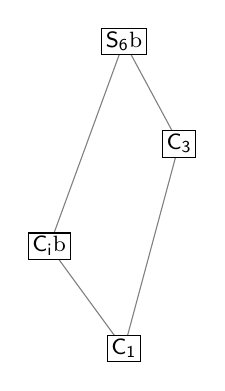
\begin{tikzpicture}[x=1cm, y=1.300cm,
  every node/.style={fill=white, font=\footnotesize, inner xsep=1.5pt, inner ysep=1.2pt, text height=5.6pt, text depth=1.6pt},
  normal/.style={draw, line width=0.4pt}, cover/.style={black!50, line width=0.4pt}]
\draw[cover] (0.00,0) -- (-0.95,1);
\draw[cover] (0.00,0) -- (0.70,2);
\draw[cover] (-0.95,1) -- (0.00,3);
\draw[cover] (0.70,2) -- (0.00,3);
\node[normal] (n00) at (0.00,0) {$\grp{C_{1}}$};
\node[normal] (n01) at (-0.95,1) {$\grp{C_{i}}\secondclass$};
\node[normal] (n02) at (0.70,2) {$\grp{C_{3}}$};
\node[normal] (n03) at (0.00,3) {$\grp{S_{6}}\secondclass$};
\end{tikzpicture}
\end{center}
{\small\setlength{\fillwidth}{\textwidth}\addtolength{\fillwidth}{-12\tabcolsep}\setlength{\colwidth}{0pt}\cellmax{subgrp}\cellmax{$\grp{C_{i}}\secondclass$}\cellmax{$\grp{S_{6}}\secondclass$}\cellmax{$\grp{C_{1}}$}\cellmax{$\grp{C_{3}}$}\addtolength{\fillwidth}{-\colwidth}\setlength{\colwidth}{0pt}\cellmax{order}\cellmax{1}\cellmax{2}\cellmax{3}\cellmax{6}\addtolength{\fillwidth}{-\colwidth}\setlength{\colwidth}{0pt}\cellmax{conjugates}\cellmax{1}\addtolength{\fillwidth}{-\colwidth}\setlength{\colwidth}{0pt}\cellmax{normal}\cellmax{yes}\addtolength{\fillwidth}{-\colwidth}\setlength{\colwidth}{0pt}\cellmax{$\grp{N}_{\grp{G}}(\grp{H})$}\cellmax{$\grp{S_{6}}\secondclass$}\addtolength{\fillwidth}{-\colwidth}\setlength{\colwidth}{0pt}\cellmax{$\grp{C}_{\grp{G}}(\grp{H})$}\cellmax{$\grp{S_{6}}\secondclass$}\addtolength{\fillwidth}{-\colwidth}\setlength{\colwidth}{0pt}\cellmax{classes}\cellmax{$\cls{C_{3}}$, $\cls{C_{3}^{2}}$}\cellmax{---}\cellmax{all}\cellmax{$\cls{i}$}\fillcap\begin{longtable}{@{}lrrlll>{\RaggedRight\arraybackslash}p{\fillwidth}@{}}\toprule
subgrp & order & conjugates & normal & $\grp{N}_{\grp{G}}(\grp{H})$ & $\grp{C}_{\grp{G}}(\grp{H})$ & classes\\\midrule\endhead
\bottomrule\endfoot\endlastfoot
\href{C1.pdf}{$\grp{C_{1}}$} & 1 & 1 & yes & \href{S6b.pdf}{$\grp{S_{6}}\secondclass$} & \href{S6b.pdf}{$\grp{S_{6}}\secondclass$} & ---\\*
\href{S2b.pdf}{$\grp{C_{i}}\secondclass$} & 2 & 1 & yes & \href{S6b.pdf}{$\grp{S_{6}}\secondclass$} & \href{S6b.pdf}{$\grp{S_{6}}\secondclass$} & $\cls{i}$\\
\href{C3.pdf}{$\grp{C_{3}}$} & 3 & 1 & yes & \href{S6b.pdf}{$\grp{S_{6}}\secondclass$} & \href{S6b.pdf}{$\grp{S_{6}}\secondclass$} & $\cls{C_{3}}$, $\cls{C_{3}^{2}}$\\*
\href{S6b.pdf}{$\grp{S_{6}}\secondclass$} & 6 & 1 & yes & \href{S6b.pdf}{$\grp{S_{6}}\secondclass$} & \href{S6b.pdf}{$\grp{S_{6}}\secondclass$} & all\\
\bottomrule\end{longtable}}
\needspace{171pt}
\partbox{Spinors and tensors}
\section{Invariant polynomials}\label{s:invariants}
Conventions: \href{../../CONVENTIONS.pdf}{CONVENTIONS.pdf}, section \href{../../CONVENTIONS.pdf\#conv.26.4}{26.4}.
\leavevmode\label{n:local.spinor.uv}\label{n:local.binary.form}A binary form $f = \sum_i c_i\, u^i v^{n-i}$ of degree $n$ in the spin kets $u = \jm{1/2}{1/2}$ and $v = \jm{1/2}{-1/2}$ is invariant when $k f = f$ for every element $k$, the elements acting at the parity $+1$ (\href{../../CONVENTIONS.pdf}{CONVENTIONS.pdf}, section \href{../../CONVENTIONS.pdf\#conv.26.4}{26.4}); at the parity $-1$ the invariants of odd degree are the semi-invariants of $\det_{\grp{G}}$ and those of even degree the same.
\leavevmode\label{n:function.hilbert}The matrices of the elements on $u$, $v$ form the cyclic group of order 6 about $z$, whose invariant forms [\href{../../../REFERENCES.pdf\#ref.Kle84}{Kle84}] are the polynomials in $uv$, $u^{6}$ and $v^{6}$, with the one relation $(uv)^{6} = u^{6}v^{6}$, their number in degree $n$ the coefficient of $t^n$ in $H(t) = (1 + t^{6})/((1-t^{2})(1-t^{6}))$, and the semi-invariants are the sums of monomials $u^i v^{n-i}$ on which the elements act alike. A section has no spinor irreps (\href{../../CONVENTIONS.pdf}{CONVENTIONS.pdf}, section \href{../../CONVENTIONS.pdf\#conv.27}{27}), so its record has no Molien series of spinor irreps: its irreps have dimension 1, and the invariants of one whose values are the $m$-th roots of unity are the powers of the $m$-th power of its partner.
\end{document}
